\PassOptionsToPackage{activate=false,expansion=false,protrusion=false}{microtype}
\documentclass[a4paper,num-refs,gigabyte]{oup-contemporary}

\journal{gigabyte}

\microtypesetup{expansion=false}
\usepackage{graphicx}
\usepackage{siunitx}

\title{Segovia v0.4.1: a bounded-memory, near-real-time streaming preprocessor for Neuropixels-scale electrophysiology}

\author[1,\authfn{1}]{Felipe Carvajal Brown}

\affil[1]{Independent Researcher}

\authnote{\authfn{1}fcarvajalbrown@gmail.com; ORCID 0000-0002-8300-7587}

\papercat{Technical Release}

\runningauthor{Carvajal Brown}

\jvolume{00}
\jnumber{0}
\jyear{2026}

\begin{document}

\begin{frontmatter}
\maketitle
\begin{abstract}
Segovia is an open-source Rust library with Python bindings for bounded-memory, near-real-time preprocessing of high-density extracellular electrophysiology recordings. It applies a bandpass-filter, common-median-reference, and whitening chain to Neuropixels-scale (384--768 channels, 30 kHz) 16-bit integer streams one chunk at a time, releasing the Python Global Interpreter Lock for each Rust computation. Peak memory is bounded by chunk size, not by recording length, and scales analytically. On a full 55.8-minute International Brain Laboratory AP-band recording (385 channels, mtscomp-compressed) at a 300 ms chunk budget, Segovia holds 99.7\% real-time deadline adherence at 0.21 GB peak resident memory. The package ships three production readers (SpikeGLX, Zarr, mtscomp) and a built-in streaming synthetic simulator.

\textbf{Availability and Implementation:} Source code (Rust and Python, AGPL-3.0-or-later): \url{https://github.com/fcarvajalbrown/Segovia}. Install via \texttt{pip install segovia} (PyPI) or \texttt{cargo add segovia} (crates.io). Version v0.4.1.
\end{abstract}

\begin{keywords}
electrophysiology; Neuropixels; streaming; real-time preprocessing; bounded memory; Rust; spike sorting
\end{keywords}
\end{frontmatter}

\section{Statement of Need}
\label{sec:background}

Neuropixels probes \citep{Jun2017} acquire 384 channels at 30 kHz ($\sim$22 MB/s per probe). Standard preprocessing pipelines (SpikeInterface \citep{Buccino2020}, MountainSort) run offline on completed recordings and are optimized for batch throughput. Near-real-time applications, such as closed-loop stimulation and online brain-machine interface decoding, require that each incoming chunk of samples be preprocessed within its acquisition period (the real-time deadline), with peak memory independent of recording length. Batch tools driven one chunk at a time re-read filter-margin neighbourhoods on every call and do not bound memory analytically. Segovia was built to fill this gap: a composable streaming preprocessor whose memory ceiling is fixed by chunk size and whose per-chunk latency meets the acquisition deadline on real recordings.

Existing ecosystems illustrate the gap. SpikeInterface \citep{Buccino2020} unifies sorters such as MountainSort \citep{Chung2017} and Kilosort \citep{Pachitariu2024} behind a common API, but its preprocessing is oriented to offline batch runs over completed recordings. Dedicated real-time neuroscience platforms exist, including improv \citep{Draelos2025}, BRAND \citep{Ali2024}, and RT-Sort \citep{vanderMolen2024}, but they target closed-loop experiment orchestration or online detection-and-sorting rather than a reusable, memory-bounded streaming preprocessor that other pipelines can compose. Segovia occupies that niche as a small primitive any of these systems could drive.

\section{Implementation}

\subsection{Core abstraction}

Segovia's \texttt{ChunkSource} trait is an iterator over fixed-size (samples $\times$ channels) 16-bit integer buffers. Three production implementations are provided:

\begin{itemize}
\item \texttt{SpikeGlxReader}: memory-mapped SpikeGLX \texttt{.bin} + \texttt{.meta} (zero-copy).
\item \texttt{ZarrReader}: chunked Zarr arrays (gzip, zstd, Blosc) via the \texttt{zarrs} crate.
\item \texttt{CbinReader}: mtscomp-compressed IBL \texttt{.cbin}, per-chunk zlib decompression via \texttt{flate2}.
\end{itemize}

\subsection{Preprocessing chain}

\texttt{preprocess(chunk\_source, config)} applies a Rayon-parallelized chain: a 5th-order Butterworth bandpass filter (zero-phase \texttt{sosfiltfilt}), common median reference, and global ZCA whitening. The Python GIL is released via PyO3's \texttt{allow\_threads} for the Rust computation. Cross-chunk IIR filter state is maintained deterministically regardless of thread count.

Peak resident memory scales as $\mathrm{batch} \times (\mathrm{chunk} + 2\,\mathrm{margin}) \times \mathrm{channels} \times \mathrm{sizeof}(f32)$ and is independent of recording length. The default (auto) batch width is capped at $\min(\mathrm{logical\ threads}, 4)$ as a conservative out-of-memory guard, bounding the default footprint to $\sim$1.2 GB on any machine; callers may pin an explicit batch. This cap is an out-of-memory safety guard, not a throughput-optimum claim.

\subsection{Built-in simulator}

\texttt{SyntheticEphysReader} emits arbitrarily long synthetic streams without writing to disk. Spike templates use a Ricker temporal waveform with point-source spatial decay ($V(r) = A\,d_\perp / r$); firing is Poisson per unit; noise is additive white Gaussian. The pseudorandom number generator (SplitMix64 + xoshiro256++) is platform-independent and chunk-size-independent. \texttt{ground\_truth()} returns (sample, unit, channel) tuples for downstream sorter evaluation.

\subsection{Testing and validation}

Correctness is covered by 38 Rust unit tests, spanning the DSP operators, the three readers, and the two simulators, and 39 Python integration tests under \texttt{tests/}. Each reader is validated to produce byte-identical output against reference recordings, and the preprocessing chain is validated against a whole-signal SciPy reference. The simulators' dependency-free Rust RNG yields bit-identical, chunk-size-independent output across platforms. Continuous integration (GitHub Actions) runs formatting, Clippy lints, and the full test suite on every push, alongside a wheel-build matrix across Linux, macOS, and Windows.

\section{Results}

Evaluation follows a replay-at-acquisition-rate methodology: data are streamed at the true 30 kHz rate with per-chunk compute latency measured by a monotonic clock. Deadline adherence is the fraction of chunks with latency at or below the chunk period.

Figure~\ref{fig:latmem} and Table~\ref{tab:fulllength} report the full-length steady-state comparison. At steady state Segovia leads on every axis; the decisive margins are peak memory (2$\times$), maximum latency (2.8$\times$), and jitter. Table~\ref{tab:coldstart} is the cold-start first-60 s window, where SpikeInterface's warm-up cost is highest and the adherence gap is widest (100\% vs 69.5\% at 300 ms); that gap narrows to the steady-state figures over the full recording.

\begin{figure}[t]
\centering
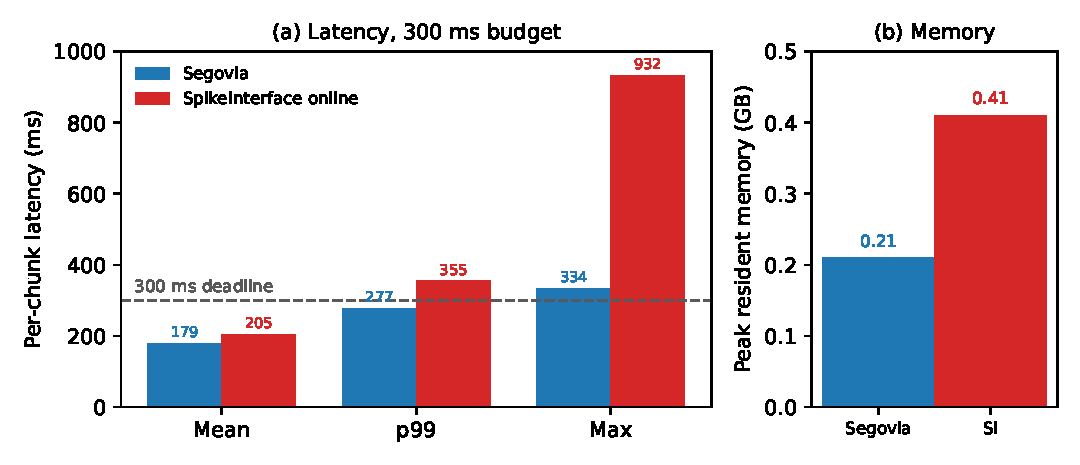
\includegraphics[width=\linewidth]{fig_latency_memory}
\caption{Full-length steady-state comparison on the real IBL AP-band recording (385 channels, 55.8 min, 300 ms budget). (a) Per-chunk latency (mean, p99, maximum) against the 300 ms real-time deadline; Segovia's maximum of 334.5 ms yields 99.7\% deadline adherence, whereas SpikeInterface online reaches 932 ms. (b) Peak resident memory, 0.21 GB versus 0.41 GB.}
\label{fig:latmem}
\end{figure}

\begin{table*}[t]
\caption{Real IBL AP-band recording, full length (385 channels, mtscomp-compressed, 55.8 min, 11{,}167 chunks, 300 ms budget, steady state).}
\label{tab:fulllength}
\begin{tabular}{l r r r r r r}
\toprule
Engine & Mean & p99 & Max & Adherence & Peak RSS & Jitter\\
\midrule
Segovia & 179.2 ms & 277.0 ms & \textbf{334.5 ms} & \textbf{99.7\%} & \textbf{0.21 GB} & \textbf{38.6 ms}\\
SpikeInterface online & 205.3 ms & 355.0 ms & 932.0 ms & 94.7\% & 0.41 GB & 60.5 ms\\
\bottomrule
\end{tabular}
\end{table*}

\begin{table*}[t]
\caption{Real IBL AP-band recording, cold-start first 60 s (385 channels, mtscomp-compressed).}
\label{tab:coldstart}
\begin{tabular}{l l r r r r}
\toprule
Chunk & Engine & Mean latency & p99 & Adherence & Peak RSS\\
\midrule
100 ms & Segovia & 92.9 ms & 122.0 ms & \textbf{74.2\%} & \textbf{0.21 GB}\\
100 ms & SpikeInterface online & 112.0 ms & 275.2 ms & 64.2\% & 0.46 GB\\
300 ms & Segovia & 194.5 ms & 256.4 ms & \textbf{100\%} & \textbf{0.28 GB}\\
300 ms & SpikeInterface online & 245.8 ms & 365.7 ms & 69.5\% & 0.52 GB\\
1000 ms & Segovia & 617.3 ms & 705.9 ms & \textbf{100\%} & \textbf{0.49 GB}\\
1000 ms & SpikeInterface online & 786.0 ms & 947.5 ms & 98.2\% & 0.74 GB\\
\bottomrule
\end{tabular}
\end{table*}

On synthetic recordings (384 channels, \texttt{SyntheticEphysReader}, seed 0) Segovia reaches 100\% deadline adherence at all chunk sizes (100/300/1000 ms) with jitter 3.6/8.6/18.6 ms.

Peak memory is bounded and file-size-independent on both sources; on the full 55.8-minute (29 GB compressed) real recording the memory bound holds to within 1\% of a ten-minute slice. In a batch-throughput comparison on that full recording, Segovia at a pinned batch held peak memory below both SpikeInterface executor modes (1.19 GB vs 2.18 GB thread-pool and 4.42 GB process-pool) and completed in less wall time (806 s vs 923 s and 1022 s) in a single run; the memory bound is the robust result and the wall-time margin warrants multi-run replication. Throughput exceeds the 22 MB/s Neuropixels acquisition rate at all configurations.

Known limitation: the zero-phase Butterworth filter introduces a 50 ms look-ahead; a causal filter mode is not yet implemented. Benchmarks are on a single machine (Windows, 8 physical / 16 logical cores).

\subsection{Reproducibility}

The benchmark harness ships in the repository: \texttt{bench/replay\_latency.py} drives Segovia and \texttt{bench/replay\_latency\_si.py} the SpikeInterface baseline, both replaying from disk at the true 30 kHz acquisition rate and timing each chunk with a monotonic clock; reported runs use a pinned batch width. Output equivalence was checked directly: with whitening disabled, Segovia matches SpikeInterface to 0.0035\% (the bandpass and common-median-reference stages are numerically equivalent). The whitened-run difference reflects SpikeInterface's random-subset whitening versus Segovia's deterministic calibration, not a discrepancy in the shared stages. Synthetic benchmarks reproduce exactly from a fixed seed.

\section{Availability of source code and requirements}

\begin{itemize}
\item Project name: Segovia
\item Project home page: \url{https://github.com/fcarvajalbrown/Segovia}
\item Operating system(s): Linux, macOS, Windows (platform independent)
\item Programming language: Rust (core, edition 2021, minimum supported Rust version 1.74); Python bindings via PyO3
\item Other requirements: Python $\geq$ 3.8 for the bindings (prebuilt abi3 wheels on PyPI); a Rust toolchain and \texttt{maturin} to build from source
\item License: AGPL-3.0-or-later (OSI-approved)
\item RRID: to be registered at SciCrunch.org prior to publication
\item bio.tools ID: not yet registered
\item Version: v0.4.1
\end{itemize}

The source code is under the AGPL-3.0-or-later license (an Open Source Initiative approved license) and is openly available in the GitHub repository above, with versioned releases on PyPI and crates.io.

\section{Availability of Test Data}

Segovia is a software library; no new experimental dataset was generated. The real recording used for evaluation is a publicly released International Brain Laboratory AP-band Neuropixels recording (\texttt{\_spikeglx\_ephysData\_g0\_t0.imec0.ap.cbin}), obtainable from the International Brain Laboratory data portal. Synthetic recordings are generated deterministically on demand by \texttt{SyntheticEphysReader} (seed-fixed, no deposit required). The form of the required GigaDB deposit for a software Technical Release is being confirmed with the editorial team.

\section{Declarations}

\subsection{List of abbreviations}

AGPL: GNU Affero General Public License; AP: action potential (band); CMR: common median reference; GIL: Global Interpreter Lock; IBL: International Brain Laboratory; IIR: infinite impulse response; RSS: resident set size; SOS: second-order sections; ZCA: zero-phase component analysis (whitening).

\subsection{Ethical Approval}

Not applicable. No human or animal data were collected for this work; the recording used for evaluation is a publicly released dataset.

\subsection{Competing Interests}

The author declares that they have no competing interests.

\subsection{Funding}

No funding was received for this work.

\subsection{Author's Contributions}

F.C.B. is the sole author and performed all work (CRediT: conceptualization, software, methodology, investigation, writing).

\section{Acknowledgements}

The author thanks the International Brain Laboratory for the publicly available recording used in evaluation. The software is named in memory of Claudio Segovia.

\bibliography{paper}

\end{document}
